\bigskip 
\bigskip 
\subsubsection{Contenido}
\bigskip 
%\begin{wrapfigure}{r}{0.5\textwidth}
%  \begin{center}
%    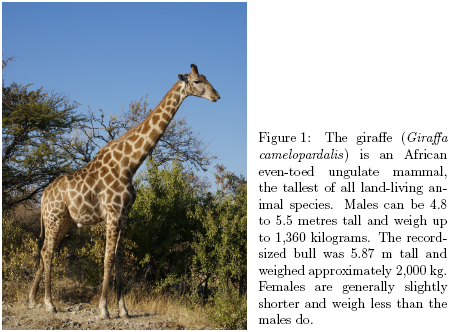
\includegraphics[width=0.48\textwidth]{./ingles/Latex_example_sidecap.jpg}
%  \end{center}
%\end{wrapfigure}

\begin{description}
\item[Nombre:] Sidecar
\item[Cristaleria:] Copa de cognac (5oz / 150cc)
\item[M\'etodo de elaboraci\'on:] Batido
\item[Decoraci\'on:] c\'ascara de lim\'on espiralada
\end{description}

\begin{table}[h]
\caption{Ingredientes y proporciones} 
\label{tab:fonts}
\begin{center}       
\begin{tabular}{|l|l|l|c|l|} %% this creates two columns
%% |l|l| to left justify each column entry
%% |c|c| to center each column entry
%% use of \rule[]{}{} below opens up each row
\hline
\rule[-1ex]{0pt}{3.5ex}  \textbf{Producto} & \textbf{Bebida} & \textbf{Marca} & \textbf{Volumen} & \textbf{Fracci\'on}  \\
\hline
\rule[-1ex]{0pt}{3.5ex}  Brandy		& Cognac			& Hennessy		 		& 1  $\frac{1}{2}$ oz / 45 cc 	&  	\\
\hline
\rule[-1ex]{0pt}{3.5ex}  Licor 		& Triple Sec 	& Cointreau 				& $\frac{3}{4}$ oz / 37,5 cc 		&  	\\
\hline
\rule[-1ex]{0pt}{3.5ex}  Fruta 		& Lim\'on	 	& Jugo	 				& 3 oz / 60 cc					& 	\\
\hline
\end{tabular}
\end{center}
\end{table} 
\bigskip 

%%-----------------------------------------------------------
\subsubsection{Formato de elaboraci\'on} 
\label{sec:title}
\bigskip 
\begin{center}
\begin{enumerate}
\item Impregnar el borde del vaso de cognac en az\'ucar.
\item Colocar hielo en una coctelera.
\item Colocar el triple sec, el cognac y el jugo de lim\'on en la coctelera y batir.
\item Servir en el vaso de cognac.
\item Decorar con la tira de c\'ascara de lim\'on.
\end{enumerate}
\end{center}
\bigskip 
\bigskip 
%%%%%%%%%%%%%%%%%%%%%%%%%%%%%%%%%%%%%%%%%%%%%%%%%%%%%%%%%%%%%

\subsubsection{Notas}
\bigskip 
\begin{center}
\raggedright{}Servir sin sorbete.
\end{center} 

\subsubsection{Informaci\'on extra}
\bigskip
\begin{center}
\medskip 
\raggedright{ \textbf{Or\'igenes de este trago}} \\ 
\medskip

{\justifying{
\indent La creaci\'on del cocktail se le atribuye a Harry MacElhone (tambi\'en creador del Brandy Alexander o el White Lady) a finales de la primera Guerra Mundial.
Se comenta que el nombre del cocktail surge por un capit\'an del ej\'ercito que todas las noches ped\'ia esta bebida para combatir el resfriado y el fr\'io, sus efectos eran tan fuertes que ten\'ian que llevarlo a su casa en Sidecar. \\

\indent Son varios los que se atribuyen la creaci\'on de este cocktail, el propio MacElhone en su libro Harry’s ABC of Mixing Cocktails le atribuy\'o el m\'erito a Pat MacGarry, un barman londinense. Tambi\'en el Hotel Ritz reclama la creaci\'on del Sidecar.
}\par}
\end{center}